\documentclass[11pt,a4paper]{article}

\usepackage[T1]{fontenc}
\usepackage[utf8]{inputenc}
\usepackage{lmodern}
\usepackage[margin=2.2cm]{geometry}
\usepackage{microtype}
\usepackage{amsmath}
\usepackage{graphicx}
\usepackage{booktabs}
\usepackage{xcolor}
\usepackage[numbers,sort&compress]{natbib}
\usepackage[colorlinks=true,linkcolor=blue!50!black,citecolor=blue!50!black,urlcolor=blue!50!black]{hyperref}

\title{Do Generated Trains Make Up for Delays?\\
\large Delay Carry-Over and Recovery in Real and LLM-Generated Train Trips}
\author{Volker Pernice \and Claude (Anthropic)}
\date{\today}

\begin{document}
\maketitle

\begin{abstract}
Generated operational records may reproduce only the structure their author expects and miss crucial details. We test this on train delays. The obvious structure is that delays carry over between stops; but trains also try to recover time. We give claude-haiku-4-5 and claude-sonnet-5 a station list and timetable of 300 real train trips and ask for actual times. We expected the models to miss both, and a prompt with carry-over to fix only carry-over. As it turns out, even without specific instruction, LLMs reproduce carry-over: generated delays are as correlated between stops as real ones (0.85 and 0.84 vs 0.88). Recovery is missed: generated trips reduce accumulated delay less often than real ones. A prompt meant to fix delay carry-over instead introduces side effects. Sonnet's delays become less correlated between stops (0.66 vs 0.88) while it recovers more often than real trips, and Haiku's delays increase.

 The planned contrast fails, but the anticipation that real, but unexpected structure is not generated holds: We observed that real delays rise suddenly and fall gradually - an incident can add any delay at once, but a train wins time back only as fast as its schedule slack allows. Over all trips, delay rises by 3 minutes or more at 1.5\% of stop-to-stop changes and falls by as much at 0.7\%. Generated delays change in small steps: with either prompt, both models produce large rises (3 minutes or more) at no more than 1.1\% of stop-to-stop changes and large falls at no more than 0.2\%. This is the kind of structure real data adds - it comes from operational constraints that neither the model nor the prompt writer considers.
\end{abstract}

\section{Question}
As is well known, LLMs are poor samplers of distributions \citep{zhang2024forcing,zhao2026dice} and miss dependencies between columns in synthetic tables \citep{xu2024tables}. We want to show that LLMs struggle to generate realistic sequential structure, that prompts can fix that, but only what is expected and previously known. Our example scenario consists of train delays. 
Train delays carry over: a train that leaves one station late tends to leave the next one late. Additionally, timetables contain slack, so a late train is able to make up time between stops. An agent that monitors a network, rebooks passengers or predicts arrival times needs to consider both. Carry-over tells it that a delay will last; recovery tells it how fast the delay shrinks.

If a generative model for synthetic operational records only knows about carry-over, agents trained or evaluated on its trips expect correlated delays but may not be able to devise recovery strategies. 

\section{Hypotheses}

Delay correlation is the lag-1 Pearson correlation of delays at consecutive stops, pooled over all steps of all trips. Recovery is the share of consecutive-stop steps where the delay decreases. A neutral prompt asks for realistic records; the instructed prompt adds that delays carry over. Intervals are paired bootstrap 95\% intervals over trips (Section~\ref{sec:method}).

We expected that without instruction, LLMs miss both carry-over and recovery, and that when told delays carry over, they fix carry-over but still miss recovery. Recovery stands in for structure the prompt writer does not name.

\textbf{H1.} With a neutral prompt, LLM-generated trips have lower delay correlation than real trips. Falsified unless the interval of the difference (neutral minus real) lies entirely below 0.

\textbf{H2.} With a neutral prompt, LLM-generated trips recover less often than real trips. Supported if the interval of the recovery difference (neutral minus real) lies entirely below 0.

\textbf{H3.} The instructed prompt closes the correlation gap but not the recovery gap. Supported if the interval of the correlation difference (instructed minus real) contains 0 and the interval of the recovery difference excludes 0.

All three can fail: models may have seen delay statistics, and the instruction could teach recovery as a side effect.

\section{Method}
\label{sec:method}

\paragraph{Real data.} We use the Rijden de Treinen archive of live departure information from Nederlandse Spoorwegen (NS), the Dutch national rail operator, for June 2025 \citep{rdt2025archive}. It holds 108{,}441 Intercity and Sprinter services, with one row per stop, scheduled times and whole-minute delays. A trip vector holds the departure delay at every stop but the last and the arrival delay at the last. We keep services that were neither completely nor partly cancelled, have at least 5 stops and have a delay wherever the trip vector needs one. From these we sample 150 Intercity and 150 Sprinter trips (seed 0).

\paragraph{Generated data.} For each real trip the model receives its skeleton: type, train number, date, and a CSV of stations with scheduled arrival and departure (HH:MM). It returns actual arrival and departure times per stop as CSV. Route, length and schedule are fixed, so only delays can differ. We call the real trip the generation's real twin. The \emph{neutral} prompt opens with ``Generate realistic operational records for this train service.'' The \emph{instructed} prompt adds ``Delays carry over from one stop to the next.'' The system prompt fixes only the output format. We run claude-haiku-4-5 (Haiku) and claude-sonnet-5 (Sonnet) with default sampling, through the Claude Agent SDK without tools. Each arm (one model with one prompt) gets one call per trip. Generated delay is actual minus scheduled time, wrapped across midnight.

\paragraph{Validity.} A generation is invalid if its row count or station names differ from the skeleton, a needed time is not HH:MM, or the train departs before it arrives. We drop invalid generations together with their real twins.

\paragraph{Control.} Shuffling each real trip's delays keeps the delay distribution and destroys order. Delay correlation must drop on the shuffled trips, or it does not measure order.

\paragraph{Metrics and significance.} We also report three descriptive metrics: the share of unchanged steps; the share of zero-delay stops; and the share of delays $\ge 5$ minutes. The last two separate a wrong distribution from a wrong order. Stops within a trip are correlated, so we resample trips, not stops. We draw 1{,}000 resamples of trip IDs with replacement, keeping twins paired, and take the difference arm minus real on the pooled steps of each. Intervals are the 2.5th and 97.5th percentiles.

\section{Results}

Two of 300 generations were invalid in each Haiku arm, none in the Sonnet arms. The control passed: shuffling lowers delay correlation from 0.88 to 0.61 (difference $-0.27$, $[-0.40, -0.17]$). Table~\ref{tab:results} gives all metrics.

\begin{table}[ht]
\centering
\footnotesize
\setlength{\tabcolsep}{3.5pt}
\begin{tabular}{lcccccc}
\toprule
 & Real & Haiku neutral & Haiku instr. & Sonnet neutral & Sonnet instr. & Shuffled \\
\midrule
Delay correlation & 0.88 & 0.85 & 0.95 & 0.84 & 0.66 & 0.61 \\
 & & {\scriptsize $-.03\,[-.13,.06]$} & {\scriptsize $+.07\,[.03,.13]$} & {\scriptsize $-.05\,[-.10,.02]$} & {\scriptsize $-.22\,[-.28,-.14]$} & {\scriptsize $-.27\,[-.40,-.17]$} \\
Recovery & 0.14 & 0.08 & 0.04 & 0.04 & 0.17 & 0.18 \\
 & & {\scriptsize $-.06\,[-.08,-.04]$} & {\scriptsize $-.10\,[-.11,-.08]$} & {\scriptsize $-.10\,[-.12,-.08]$} & {\scriptsize $+.03\,[.01,.05]$} & {\scriptsize $+.04\,[.03,.05]$} \\
\midrule
Unchanged steps & 0.71 & 0.80 & 0.88 & 0.75 & 0.62 & 0.63 \\
Zero-delay stops & 0.73 & 0.22 & 0.05 & 0.07 & 0.15 & 0.73 \\
Delay $\ge 5$ min & 0.04 & 0.00 & 0.15 & 0.00 & 0.00 & 0.04 \\
\midrule
Recovery given late$^\dagger$ & 0.52 & 0.10 & 0.05 & 0.05 & 0.20 & -- \\
 & & {\scriptsize $-.42\,[-.46,-.37]$} & {\scriptsize $-.47\,[-.51,-.43]$} & {\scriptsize $-.47\,[-.51,-.43]$} & {\scriptsize $-.32\,[-.35,-.28]$} & \\
\bottomrule
\end{tabular}
\caption{Metrics on the 300 trips (298 for Haiku). Second lines: difference arm minus real twins with paired bootstrap 95\% interval. Delay correlation decides H1, recovery H2, both together in the instructed arms H3; the rest is descriptive. $^\dagger$Share of steps with delay $\ge 1$ at stop $k$ where the delay decreases at $k{+}1$.}
\label{tab:results}
\end{table}

\paragraph{H1 is falsified for both models.} The models handle carry-over better than we expected: neutral generations have delays as correlated as real trips. The difference is $-0.03$ $[-0.13, 0.06]$ for Haiku and $-0.05$ $[-0.10, 0.02]$ for Sonnet.

\paragraph{H2 is supported for both models.} Without instruction, trips recover less than real ones: at 8\% (Haiku) and 4\% (Sonnet) of steps against 14\% ($-0.06$ $[-0.08, -0.04]$ and $-0.10$ $[-0.12, -0.08]$).

\paragraph{H3 is falsified for both models.} There was no correlation gap to close, and the instruction opens one: delay correlation rises for Haiku ($+0.07$, $[0.03, 0.13]$) and falls for Sonnet ($-0.22$, $[-0.28, -0.14]$). Recovery stays off the real level, in opposite directions. Haiku's recovery falls ($-0.10$, $[-0.11, -0.08]$). Sonnet's overshoots ($+0.03$, $[0.01, 0.05]$): it writes trips that build up a delay over the first stops and then work it off (Figure~\ref{fig:delay}). The instruction partly adds recovery for Sonnet, but with side effects in both models.

\begin{figure}[t]
\centering
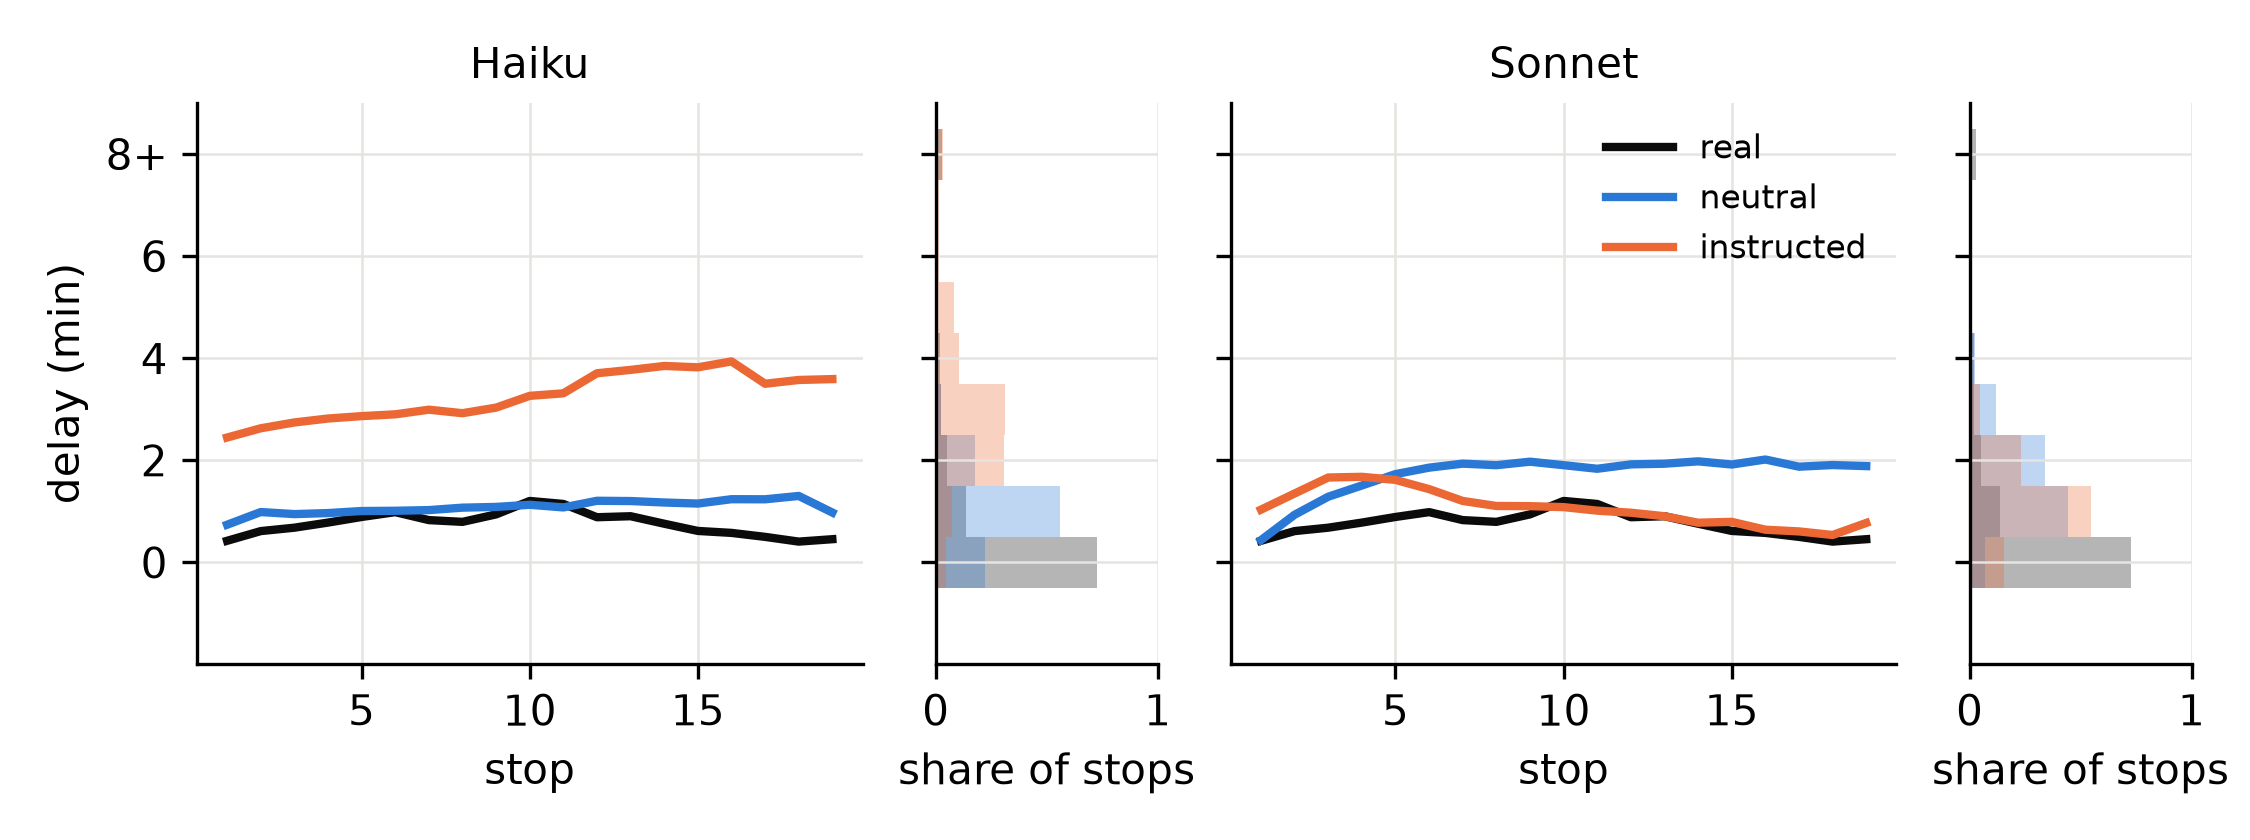
\includegraphics[width=0.56\linewidth]{../results/figures/delay_by_stop_main.png}
\caption{Mean delay by stop position (positions reached by at least 30 trips) and, at the side, share of stops at each delay (8+ pooled). Real trips (black) peak mid-route and lose delay towards the end; neutral generations (blue) hold a flat delay.}
\label{fig:delay}
\end{figure}

\paragraph{Recovery given late.} Real trains are rarely late (zero delay at 73\% of stops), so the unconditional recovery share understates the gap. Conditioned on being late (Table~\ref{tab:results}, last row), a late real train loses delay at the next stop in 52\% of steps, a late generated train in 5 to 20\%. Shuffling each generated trip raises its recovery from 0.04--0.17 to 0.17--0.27: its delays could go down, but the model writes them to hold or grow.

\paragraph{Sudden rises, gradual falls.} The planned contrast did not hold. The scatter of consecutive delays (Figure~\ref{fig:pairs}) shows a gap we did not plan for. Real delays change by large amounts, more often upwards. Over all 74{,}413 complete June trips, delay rises by 3 minutes or more at 1.5\% of steps and falls by 3 or more at 0.7\%. Large falls exist, but 85\% of falls are a single minute. Neutral generations never change a delay by more than 2 minutes in either direction. At the archive rate, their 3{,}100 steps would contain about 48 rises of 3 or more. With the instruction, Haiku writes rises of 3 or more at 1.1\% of steps and falls at 0.2\%: the sudden rise, but rarely the way back. The asymmetry has a physical cause: an incident can add any delay at once, while a train wins time back only through its schedule slack. We read the generations as following the statistics of delay records rather than the mechanics of a train; the experiment does not test this.

\begin{figure}[t]
\centering
\begin{minipage}[c]{0.5\linewidth}
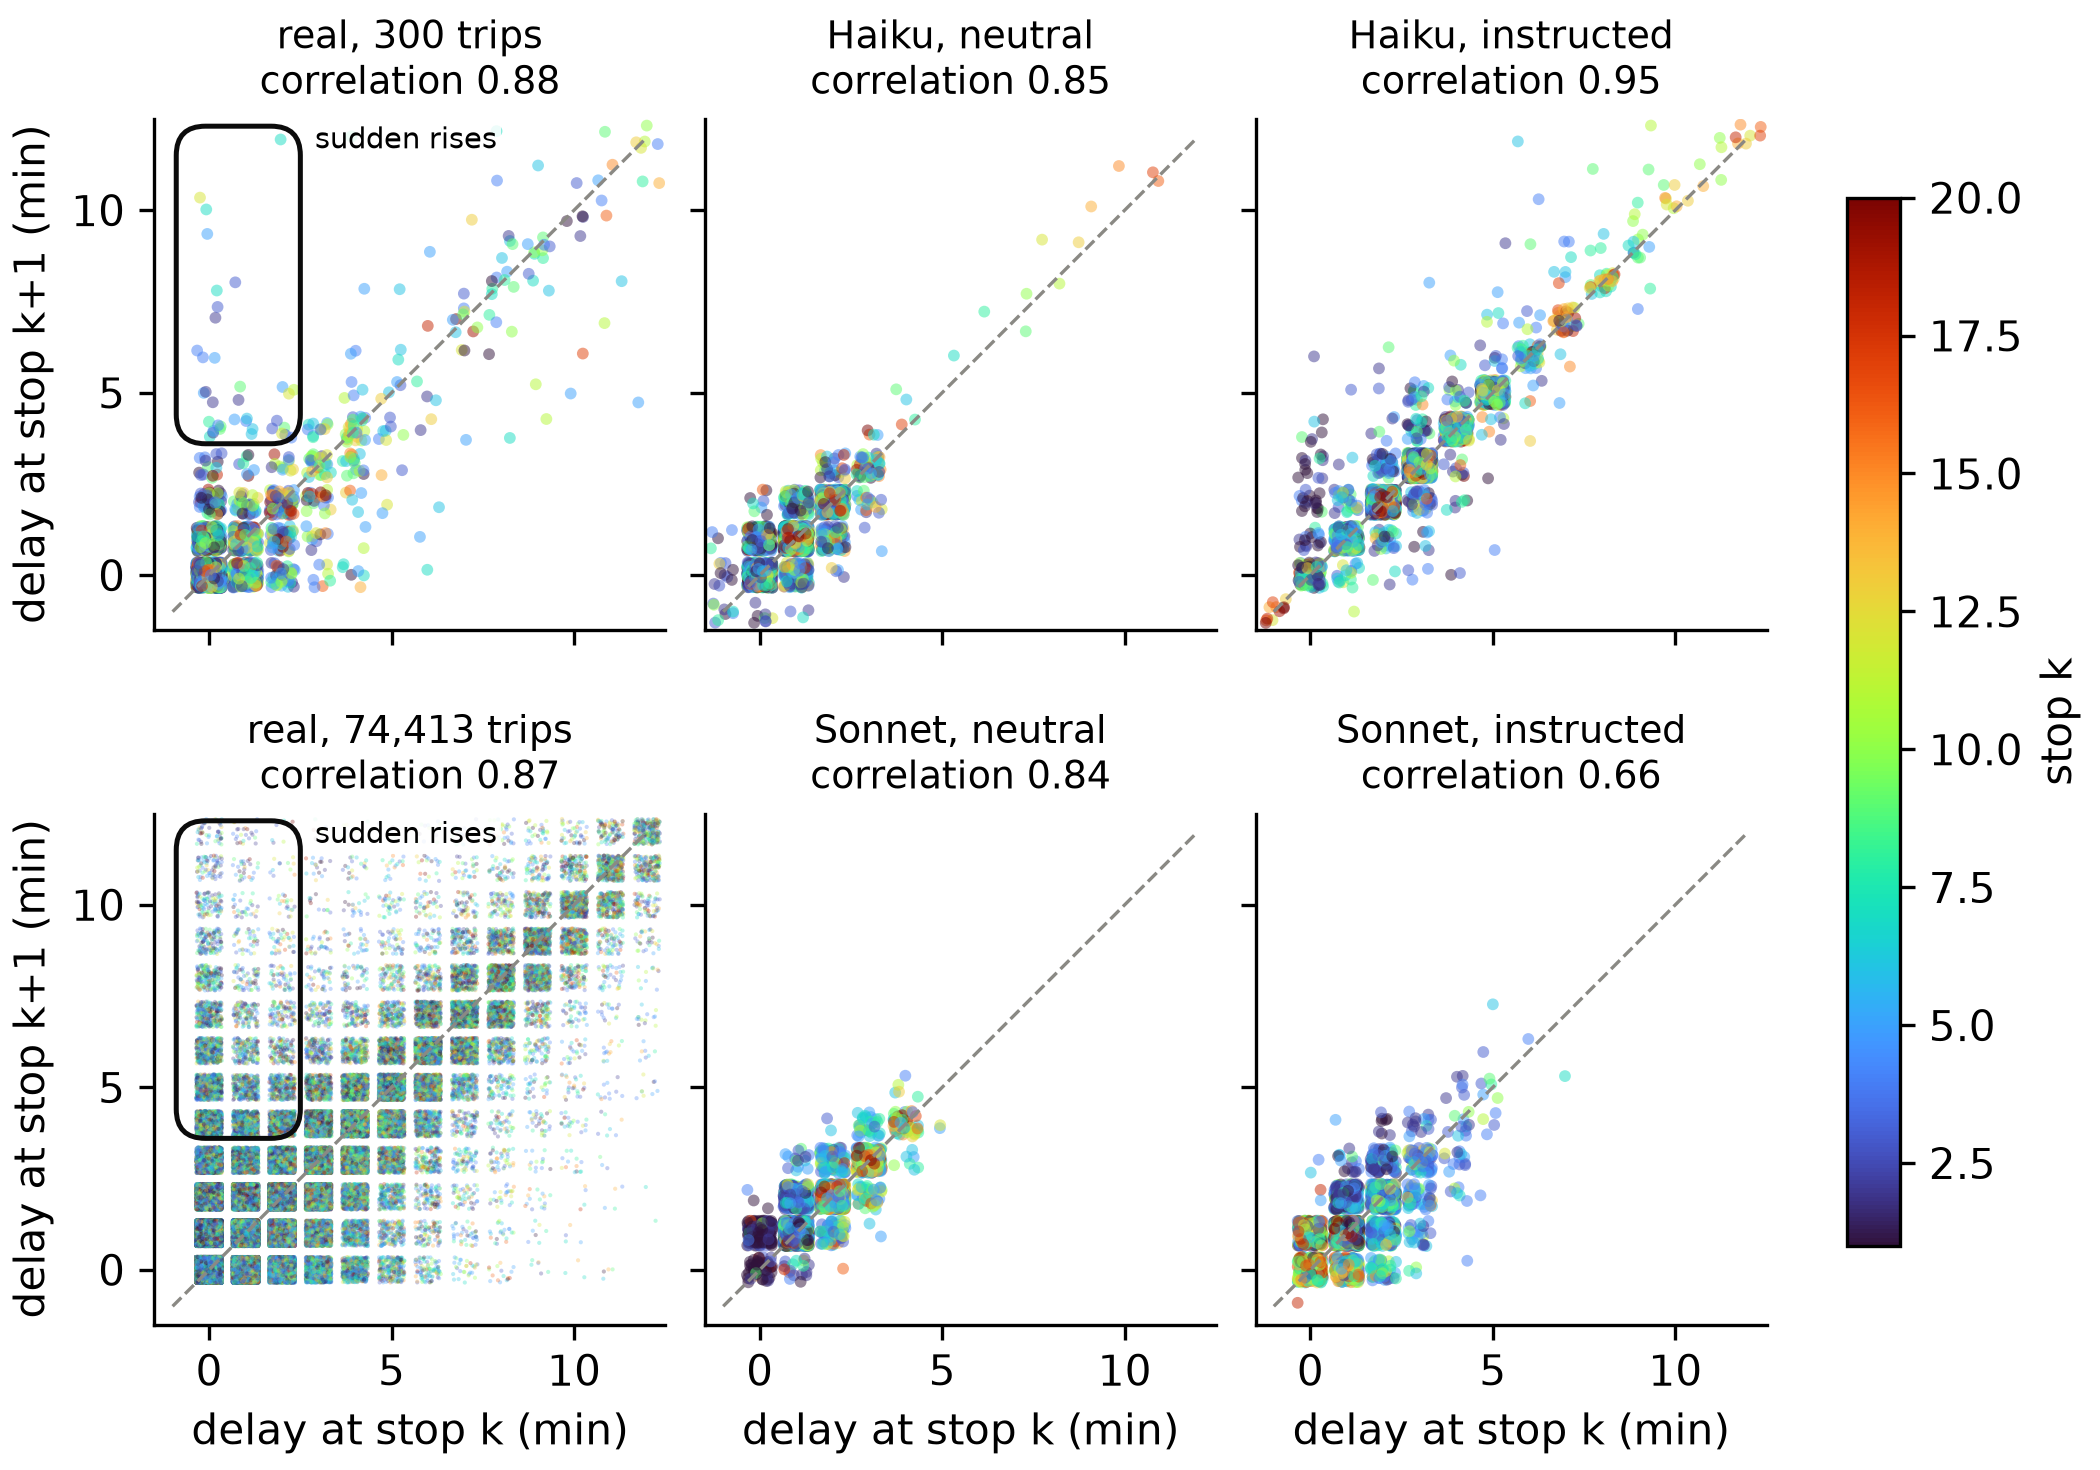
\includegraphics[width=\linewidth]{../results/figures/delay_pairs_main.png}
\end{minipage}\hfill
\begin{minipage}[c]{0.46\linewidth}
\caption{Delay at stop $k$ against stop $k{+}1$, jittered, colored by stop. First column: 300 sampled real trips (top), all complete June trips (bottom) demonstrate an asymmetric distribution. Far above the diagonal: sudden rises; far below: large falls.}
\label{fig:pairs}
\end{minipage}
\end{figure}

\section{Limits}

\paragraph{What the result does not show.} Pooled lag-1 correlation also rewards trips that are late throughout, so a generator that gives each trip one constant delay scores high on it. H1 was falsified on this metric; a within-trip measure, which we did not test, might have decided differently. Large jumps are rare. On 300 generated trips per arm, only their absence in the neutral arms is clear, and the instructed rates rest on 3 to 35 steps. Real delays come from NS live information and may be the last forecast rather than a measured time, so some sudden rises may be forecast updates. We test one operator, one month, two models from one family, one prompt pair, and default sampling through the Agent SDK (Haiku likely ran with thinking on). The rule ``interval contains 0'' for closing a gap favours small samples.

\paragraph{What real data adds, and what it only seems to add.} Recovery did not work out as our example of structure a prompt misses: the models reproduce carry-over without being told, and naming it moves recovery in unplanned ways. The jump asymmetry makes the point instead. We did not expect it, so we could neither hypothesise it nor instruct the model on it. A prompt could now name it, but only because the real data showed it. The zero-delay share is a distribution error that one prompt line (``most trains run on time'') or a resampling might fix; we did not test that. Whether the recovery gap matters could be tested downstream: fit a predictor of final delay from the delay at stop $k$, once on generated and once on real trips, and evaluate both on held-out real trips. A small error gap would mean real data only seems to add something here. Testing the general question would take this test across record types (maintenance logs, invoices, tickets) and model families, with prompts naming every known defect, to see whether what remains matters.


\renewcommand{\bibfont}{\small}
\setlength{\bibsep}{2pt}
\bibliographystyle{plainnat}
\bibliography{references}

\end{document}
